\documentclass[11pt,a4paper]{article}
\usepackage{classeRapport}
\usepackage{float}
\usepackage{algorithmeUTF8}
\usepackage{listings}


\begin{document}

    \PageDeGarde	
    {rien.png} 
    {Correcteur Orthographique} 
    {Project algorithmique} 
    {
    \textbf{Groupe 3-3}\\
    Lucile \textsc{BRUGIERE}\\
    Mohamed Mamoun \textsc{IBN-ABDELJALIL}\\
    Romain \textsc{PETITALOT}\\
    Aymane \textsc{SAHILI}} 
    {ITI3 - 2021}
    
    \Page{INSALogo}{rien.png}
    
    \clearpage 
    
    \tableofcontents
    
    \clearpage
    \section{Introduction}
    \addcontentsline{toc}{section}{Introduction}
        Dans le cadre de nos études d'ingénieur, lors de notre première anée dans le département ITI, nous avons dû 
    réaliser un projet avec pour but de concevoir un correcteur orthographique en C.\\
        
        Nous avons donc réaliser cela en utilisant le TAD FichierTexte proposé par nos professeurs et en créeant 3 autres 
    TAD : Mot, Dictionnaire et Correcteur. Le principe de notre correcteur consiste à corriger l'ensemble des mots écrits sur l'entrée standard du terminal. La correction se fait par rapport à un dictionnaire donné par nos professeurs également.\\
        
        Notre correcteur est divisé en deux grandes parties. La première concerne la construction du type Dictionnaire à partir d'un dictionnaire.txt, la conception de ce dernier est basé sur la distance de Damerau-Levenshtein qui est une version amélioré de l'algorithme de levenshtein puisqu'elle prends en compte l'inversion de deux lettres successives également.Tant dis que la deuxième partie concerne la recherche de mot dans le dictionnaire c'est-à-dire les fonctions et procédures qui permettent le parcours de notre structure Dictionnaire.\\
        
        De plus, pour respecter les consignes données par nos professeurs, nous avons ajouté la possibilité de sauvegarde du dictionnaire et d'importation de ce dernier.\\
        
        Le GIT de notre projet était géré par Romain, notre Chef de projet.
        
     
    \section{Analyse}
        \subsection{Analyse descendante}
            \subsubsection{Analyse descendante du correcteur}
            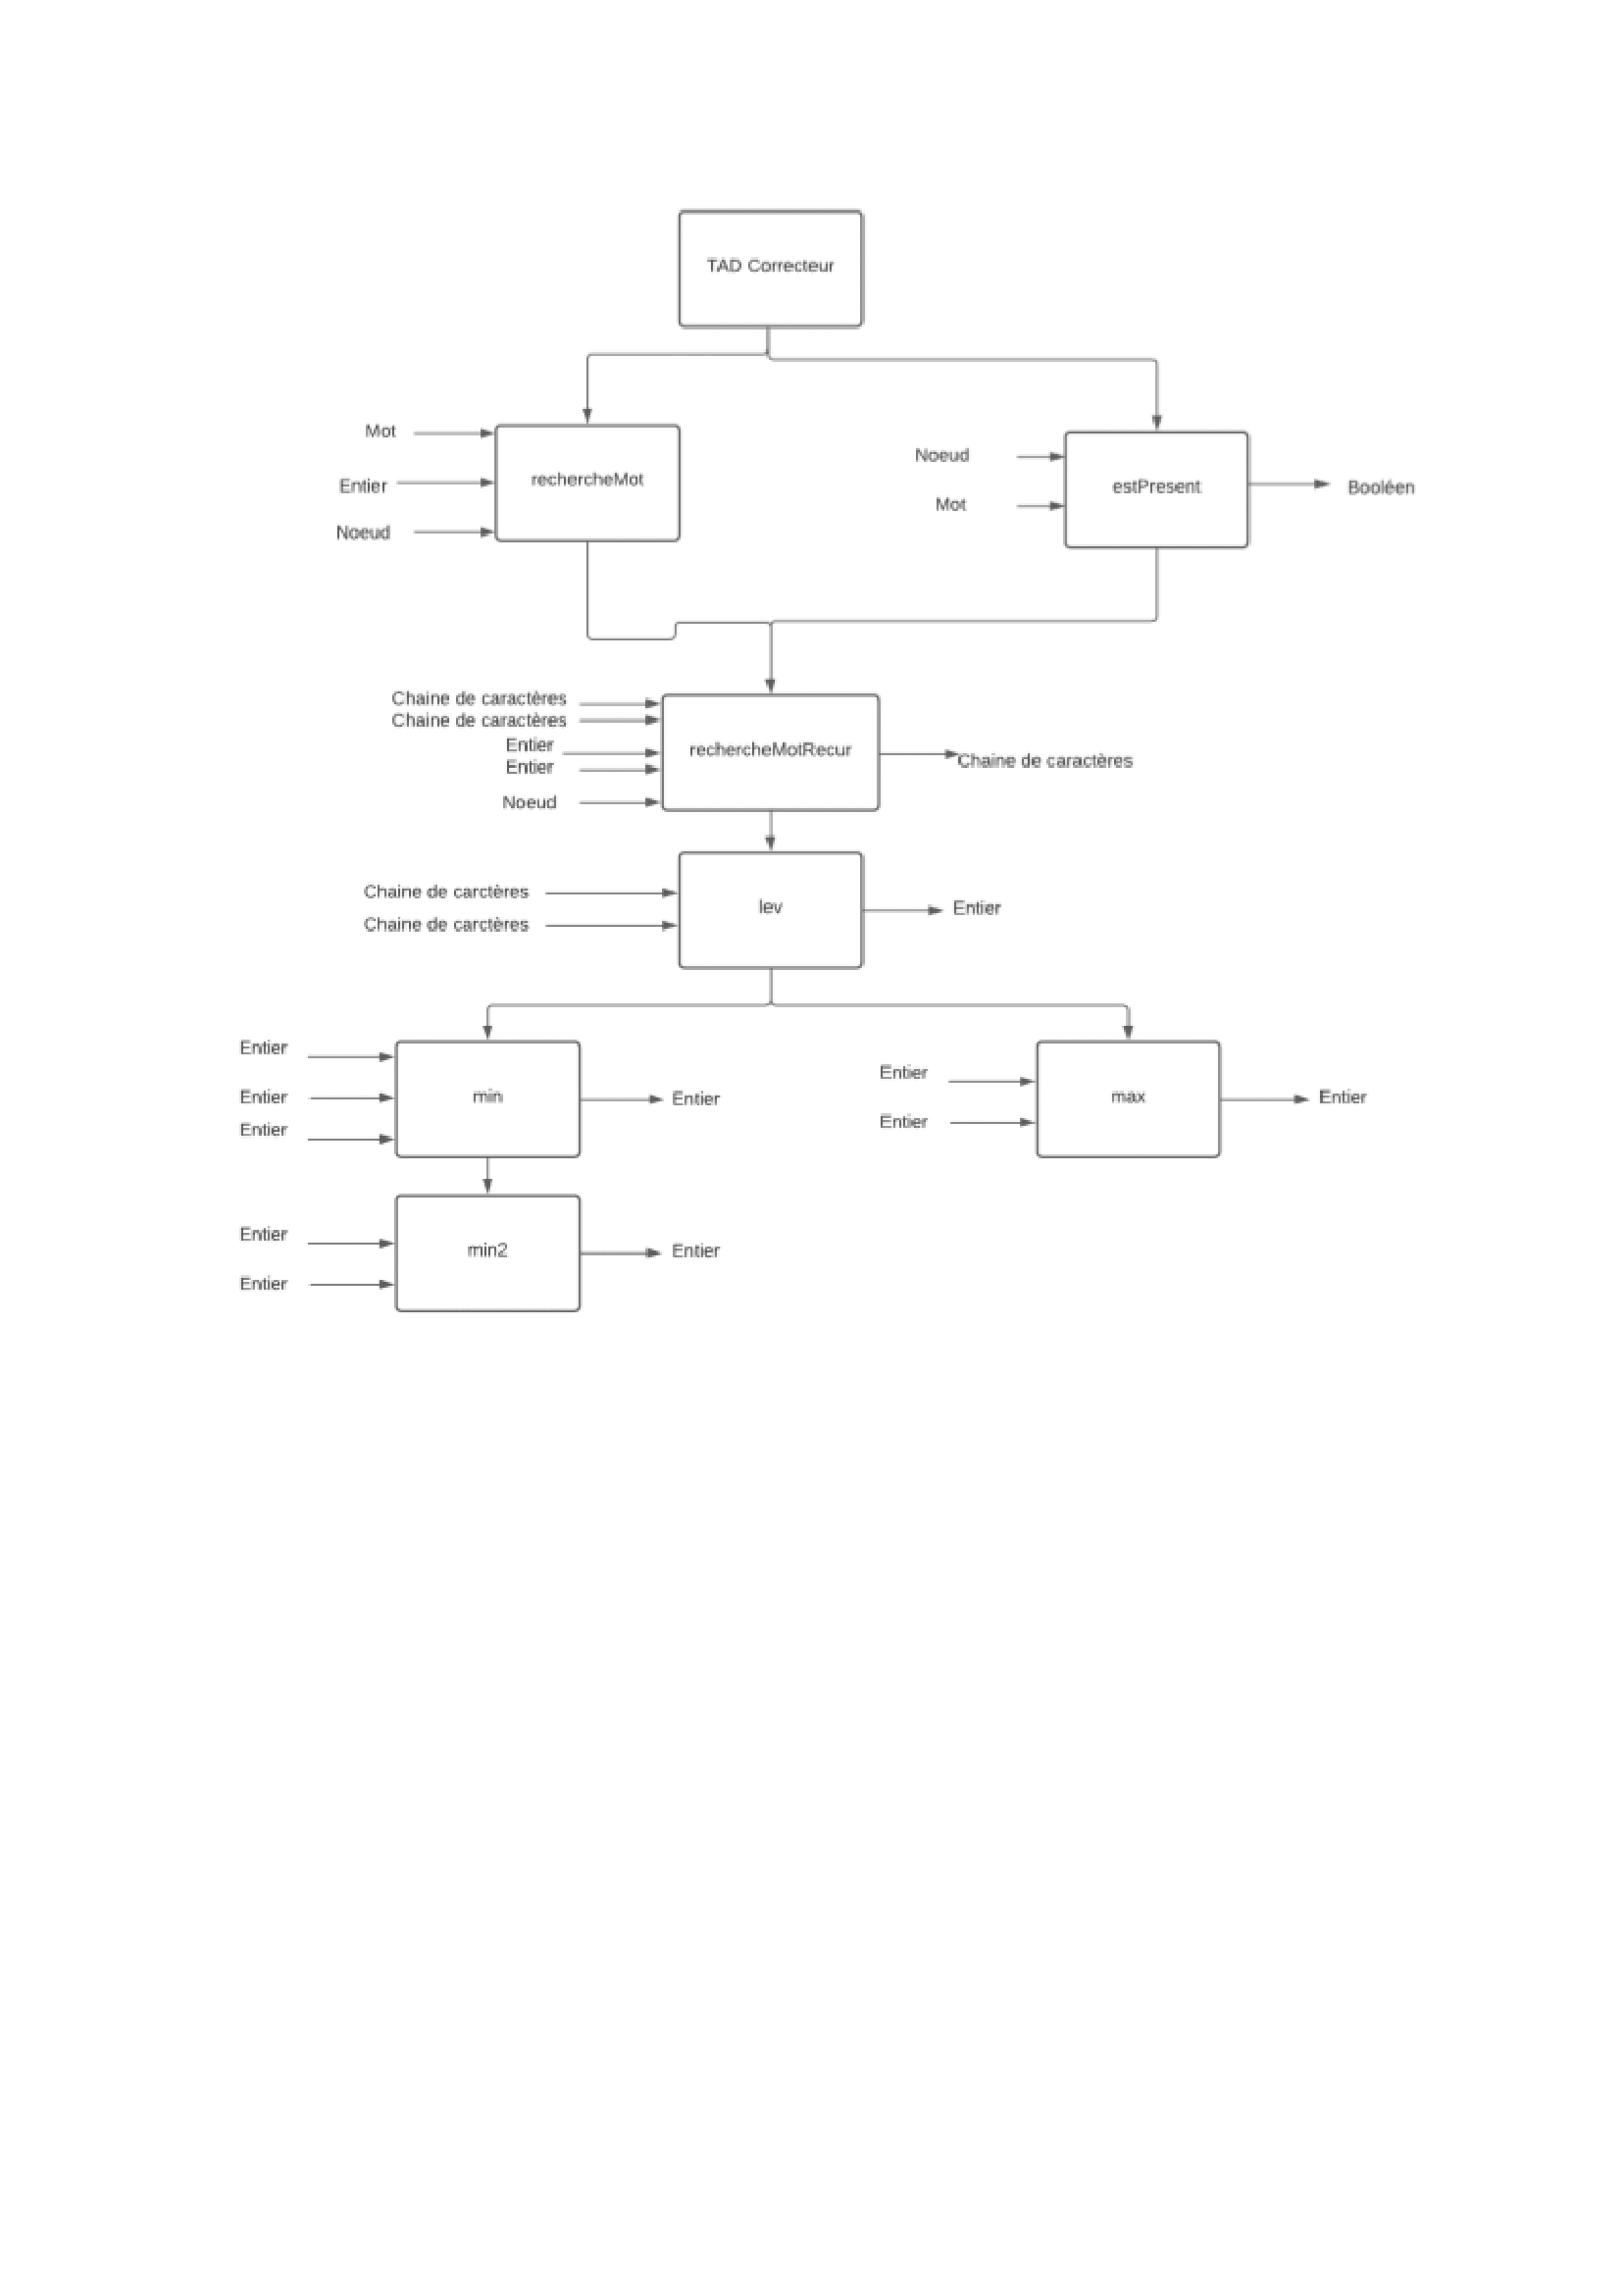
\includegraphics{images/Analyse_Descendante_Correcteur.png}
            \clearpage
            \subsubsection{Analyse descendante du dictionnaire}
            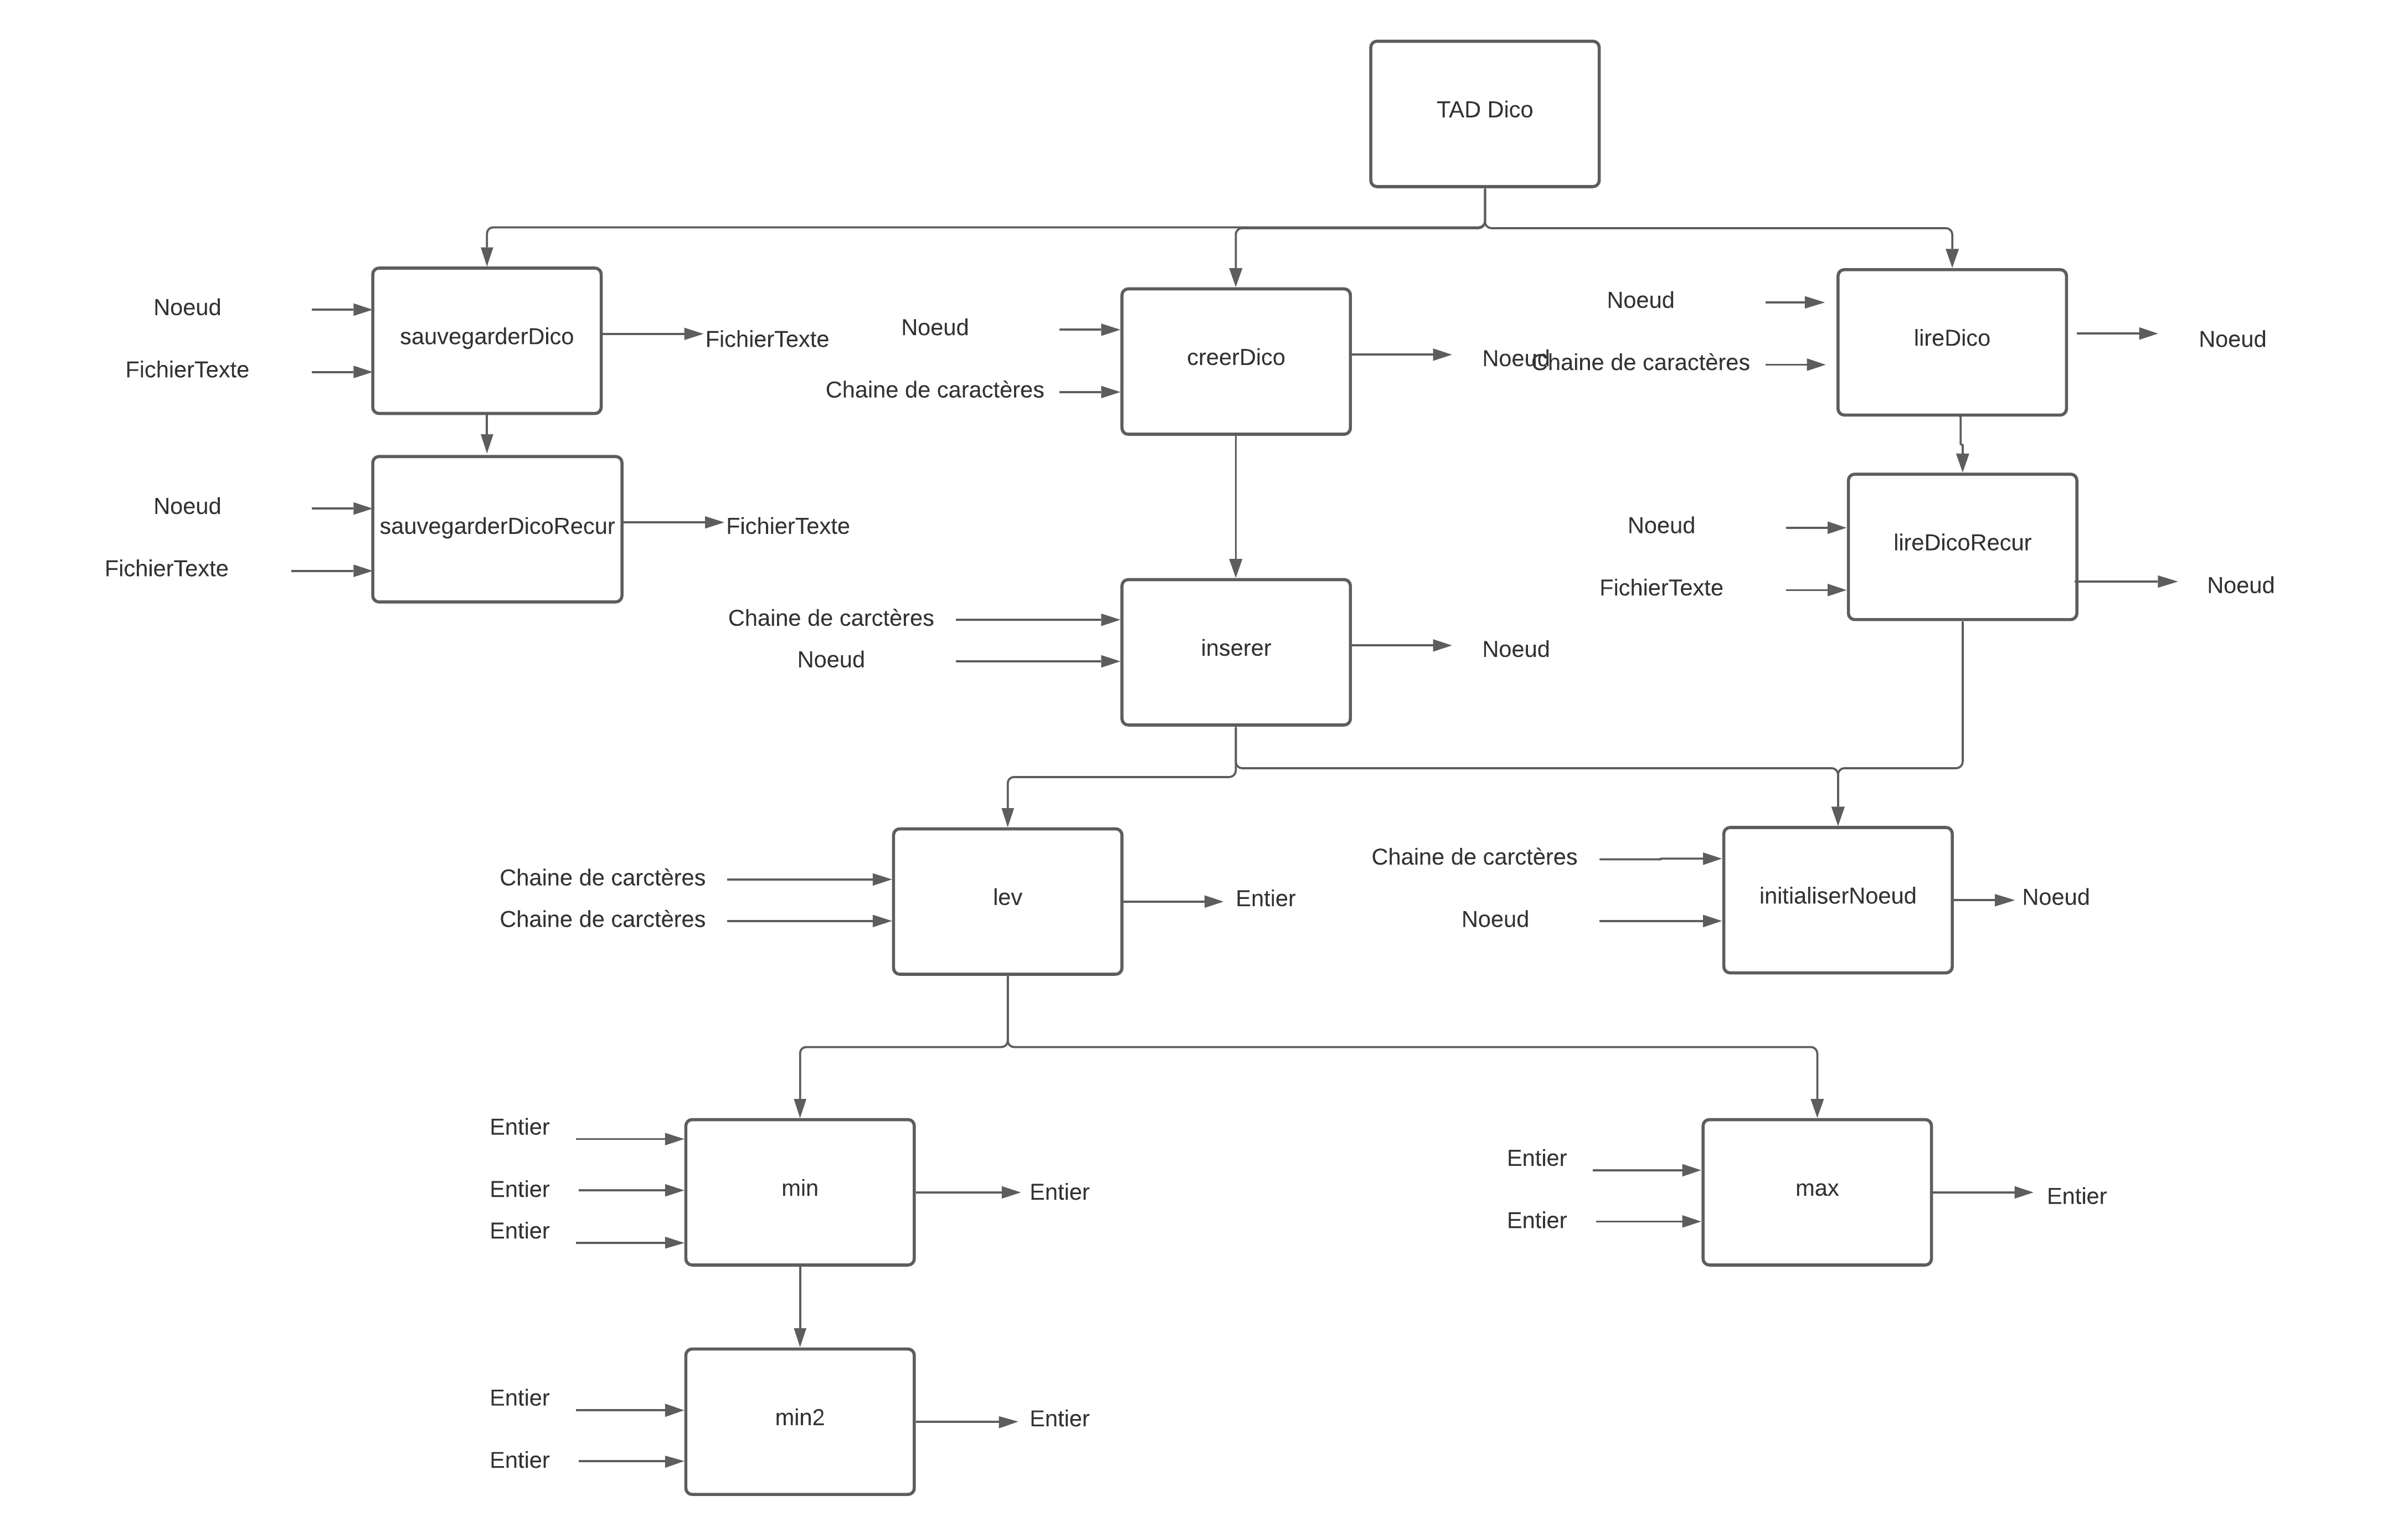
\includegraphics[scale=0.5]{images/Analyse_Descendante_Dictionnaire.png}
            \clearpage
        \subsection{Présentation des TAD}
    
                \subsubsection{Mot}

   
    \begin{tad}
        \tadNom{Mot}
        \tadDependances{Chaine de caracteres,Entier}
        
        \begin{tadOperations}{Mot}
            \tadOperation{mot}{chaine de caractères x Naturel}{\tadUnParam{Mot}}
            \tadOperation{convertirMinuscule}{Mot}{\tadUnParam{Mot}}
        \end{tadOperations}
        
        \begin{tadSemantiques}{Mot}
            
            \tadSemantique{mot}{Crée un mot à partir de sa chaine de caractères et de sa chaine lue en entrée}
            \tadSemantique{convertirMinuscule}{Convertis un mot en minuscule}
            
        \end{tadSemantiques}

        \begin{tadAxiomes}
            \tadAxiome{}
        \end{tadAxiomes}            

    \end{tad}

                \subsubsection{Correcteur}

   
    \begin{tad}
        \tadNom{Correcteur}
        \tadDependances{Mot,Dictionnaire,entier,liste}
        
        \begin{tadOperations}{Mot}
            \tadOperation{rechercheMot}{Mot x Dictionnaire x Entier}{\tadUnParam{Liste(Mot}}
            \tadOperation{estPresent}{Mot x Dictionnaire}{\tadUnParam{Entier}}
        \end{tadOperations}
        
        \begin{tadSemantiques}{dictionnaire}
            
            \tadSemantique{rechercheMot}{Cherche un mot dans le dictionnaire avec une limite donnée}
            \tadSemantique{estPresent}{Vérifie si un mot est présent dans un dictionnaire donnée}
        \end{tadSemantiques}

        \begin{tadAxiomes}
            \tadAxiome{}
        \end{tadAxiomes}            

    \end{tad}
                \subsubsection{Dictionnaire}

   
    \begin{tad}
        \tadNom{Dictionnaire}
        \tadDependances{Mot,Fichier}
        
        \begin{tadOperations}{dictionnaire}
            \tadOperation{creerArbre}{FichierTexte x Dictionnaire}{\tadUnParam{Dictionnaire}}
            \tadOperation{initialiserNoeud}{Mot x Dictionnaire}{\tadUnParam{Dictionnaire}}
            \tadOperation{inserer}{Mot x Dictionnaire}{\tadUnParam{Dictionnaire}}
            \tadOperation{sauvegarderDico}{Dictionnaire x FichierTexte}{\tadUnParam{FichierTexte}}
            \tadOperation{lireDico}{FichierTexte x Dictionnaire}{\tadUnParam{Dictionnaire}}
        \end{tadOperations}
        
        \begin{tadSemantiques}{dictionnaire}
            
            \tadSemantique{creerDico}{Crée le dictionnaire à partir d'un fichier contenant des mots corrects ligne par ligne}
            \tadSemantique{initialiserNoeud}{initialiser un dictionnaire à partir d'un dictionnaire vide et d'un mot}
            \tadSemantique{inserer}{Inserer un mot dans l'arbre}
            \tadSemantique{sauvegarderDico}{Stocke le dictionnaire dans un fichier}
            \tadSemantique{lireDico}{Charge le dictionnaire à partir du fichier où le dictionnaire a été enregistré}
        \end{tadSemantiques}

        \begin{tadAxiomes}
            \tadAxiome{creerArbre(Fichier,Dictionnaire) =  lireDico(sauvegarderDico(creerArbre(Fichier, Dictionnaire)))}
        \end{tadAxiomes}            

    \end{tad}
    

                \clearpage

    \section{Conception préliminaire}
        \subsection{Les signatures des fonctions et procédures du TAD Mot}
    \begin{algorithme}
    \signatureFonction{estPresent}
    {noeud : Noeud, chaine : Chaine de caractères}{\textbf{Booléen}}
    \end{algorithme}


        \subsection{Les signatures des fonctions et procédures du TAD Dictionnaire}

    \begin{algorithme}
    \signatureprocedure
    	{creerDico}
    	{\paramEntreeSortie {node : Noeud}; \paramEntree {filename : FichierTexte}} \\

    \signatureprocedure
    	{initialiserNoeud}
    	{\paramEntreeSortie {node : Noeud}; \paramEntree {str : Chaine de caractères}}  \\
    
    \signatureprocedure
    	{inserer}
    	{\paramEntreeSortie {node : Noeud}; \paramEntree {str : Chaine de caractères}}  \\
    	
    \signatureprocedure
    	{sauvegardeDico}
    	{\paramEntreeSortie {node : Noeud}; \paramEntree {filename : FichierTexte}}  \\

    \signatureprocedure
    	{lireDico}
    	{\paramEntreeSortie {node : Noeud}; \paramEntree {filename : FichierTexte}}  \\
    \end{algorithme}


        \subsection{Les signatures des fonctions et procédures du TAD Correcteur}
    
    \begin{algorithme}    
    \signatureProcedure{rechercheMot}
    {\paramEntree {noeud : Noeud}, \paramEntree {mot : Mot}, \paramEntree {toleranceMax : Naturel}}\\
    
    \signatureFonction{estPresent}
    {noeud : Noeud, chaine : Chaine de caractères}{\textbf{Booléen}}
    \end{algorithme}

        \clearpage

    \section{Conception détaillée}
        \subsection{Pseudo Code de Mot}
    \begin{algorithme}    
        \begin{enregistrement}{Mot}
            \champEnregistrement{chaine}{Chaine de Caractères}
            \champEnregistrement{position}{Naturel}
        \end{enregistrement}\\
    \end{algorithme}
    
    
    \begin{algorithme}    
        \fonction{initialiserMot}{chaine : Chaine de Caractère; position : Naturel}{Mot}{mot : Mot}
        {\affecter{mot.chaine}{chaine}
        \affecter{mot.position}{position}
        \retourner{mot}}
    \end{algorithme}

        \clearpage
        
        \subsection{Pseudo Code du Dictionnaire}
    
    \begin{algorithme}    
        \begin{enregistrement}{Noeud}
            \champEnregistrement{chaine}{Chaine de Caractères}
            \champEnregistrement{enfants}{tableau [1..30] de Noeud}
        \end{enregistrement}
    \end{algorithme}
    
    
    \begin{algorithme}
	\fonction
	{min2}
	{a:Entier, b:Entier}{\textbf{Entier}}
	{}
	{\sialors{a<b}{
	{\retourner{a}}}
	{\retourner{b}}
	}\\
    \end{algorithme}

    \begin{algorithme}
        \fonction
        {min}
        {a:Entier, b:Entier, c:Entier}{\textbf{Entier}}
        {}
        {\retourner{min2(a,min2(b,c))}}\\
    \end{algorithme}
    
    \begin{algorithme}
        \fonction{max}
        {a:Entier, b:Entier}{\textbf{Entier}}
        {}
        {\sialors{a>b}{\retourner{a}}
        {\retourner{b}}}\\
    \end{algorithme}
    
    \begin{algorithme}
        \fonctionAvecPreconditions{lev}
        {chaine1 : Chaine de caractères, chaine2 : Chaine de caractères}{\textbf{Entier}}
        {longueur(chaine1)<100 et longueur(chaine2)<100}
        {taille\_s1,taille\_s2,i,j,coutSubstitution : Naturel,\\ 
        mat : tableau[1..99][1..99] de Naturel}
        {{\affecter{taille\_s1}{longueur(chaine1)}}
        {\affecter{taille\_s2}{longueur(chaine2)}}
        {\pour{i}{1}{taille\_s1}{}{\pour{j}{1}{taille\_s2}{}{\affecter{mat[i][j]}{0}}}
        }
        {\pour{i}{1}{taille\_s1}{}{\affecter{mat[i][1]}{i}}
        }
        {\pour{j}{1}{taille\_s2}{}{\affecter{mat[1][j]}{j}}
        }
        {\pour{i}{1}{taille\_s1}{}{\pour{j}{1}{taille\_s2}{}
        {\sialorssinon{( chaine1[i-1]== chaine2[j-1] )}{
        {\affecter{coutSubstitution}{0}}}
        {\affecter{coutSubstitution}{1}}
        }
        {\affecter{mat[i][j]}{min(mat[i-1][j]+1,mat[i-1][j-1]+coutSubstitution,mat[i][j-1]+1)}}
        {\sialors{( i>1 et j>1 et chaine1[i-1]==chaine2[j-2] et chaine1[i-2]==chaine2[j-1] )}
        {{\affecter{mat[i][j]}{min2(mat[i][j],mat[i-2][j-2]+coutSubstitution)}}}
        }
        }
        }
        {\retourner{mat[taille\_s1][taille\_s2]}}
        }\\
    \end{algorithme}
    
    
    \begin{algorithme}
    	
    	\procedure
    	{initialiserNoeud}
    	{\paramEntreeSortie {noeud : Noeud}; \paramEntree {chaine : Chaine de caractères}} 
    	{i: Naturel}
    	{
    	{\affecter{noeud.chaine}{chaine}}
        {\pour{i}{1}{maxEnfants}{}
            {\affecter{noeud.enfants[i]}{NIL}
        }
        }
        }\\
    \end{algorithme}
    
    
    \begin{algorithme}
    	
    	\procedure
    	{inserer}
    	{\paramEntreeSortie {noeud : Noeud}; \paramEntree {chaine : Chaine de caractères}} 
    	{ld: Naturel}
    	{
    	\sialorssinon{(noeud = NIL)}{
    	\instruction{initialiserNoeud(noeud,chaine)}}
    	{\affecter{ld}{lev(noeud.chaine,chaine)}
    	 \instruction{inserer(chaine,noeud.enfants[ld])}
        }
        }\\
    \end{algorithme}
    
    
    \begin{algorithme}
    	\procedure
    	{creerDico}
    	{\paramEntreeSortie {noeud : Noeud}; \paramEntree {nom\_fichier : chaine de caractère}} 
    	{chaine : Chaine de caractères, \\ f : FichierTexte}
    	{
    	\affecter{f}{ouvrirFichier(nom\_fichier,lecture)}
    	{\instruction{lireLigne(f, chaine)}}
        {\tantque{( chaine <> EOF  )}
            {\instruction{inserer(noeud, chaine)}
            {\instruction{lireLigne(f, chaine)}}}
        }
        {\instruction{fermerFichier(f)}}
        }\\
    \end{algorithme}
    
    \begin{algorithme}
    	\procedure
    	{sauvegarderDicoRecur}
    	{\paramEntreeSortie {f : FichierTexte}; \paramEntree {noeud : Noeud}} 
    	{i: Naturel}
    	{\sialorssinon{noeud == NIL}{
    	{\instruction{ecrireDansFichier(f,"\#")}}}
    	{{\instruction{ecrireDansFichier(f, noeud.chaine)}}
    	{\pour{i}{1}{maxEnfants}{}
    	    {\instruction{sauvegarderDicoRecur(f, noeud.enfants[i])}
    	    }
    	}
    	}
        }\\
    \end{algorithme}
    
    \begin{algorithme}
    	\procedure
    	{sauvegarderDico}
    	{\paramEntree {nom\_fichier : chaine de caractère}; \paramEntree {noeud : Noeud}} 
    	{f : FichierTexte}
    	{
    	\affecter{f}{ouvrirFichier(nom\_fichier,lecture)}
    	{\instruction{sauvegarderDicoRecur(f, noeud)}}
    	{\instruction{fermerFichier(f)}}
    	}\\
  	
    \end{algorithme}
    
    
        \clearpage
        
        \subsection{Pseudo Code du Correcteur}
    
    \begin{algorithme}
        \procedure{rechercheMotRecur}
        {\paramEntreeSortie {res : Chaine de caractères}; \paramEntree {noeud : Noeud; chaine : Chaine de caractères; tolerance, counter : Naturel}}
        {i,j : Naturel}
        {\affecter{j}{lev(noeud.chaine,chaine)}
        \sialors{(j=tolerance) et (counter<6+tolerance*4)}
        {
            {
            \sialors{tolerance>0}
            {
                \instruction{concatChaine(res, noeud.chaine)}
                \instruction{concatChaine(res, " ")}
                
            }
            }
            \affecter{counter}{counter + 1}
        }
        
        {\sialors{counter < (6+tolerance*4)}
            {\pour{i}{max(1, j - tolerance)}{min(maxEnfants, j + tolerance)}{} {\instruction{rechercheMotRecur(res,noeud.enfants[i],chaine,tolerance,counter)}
        }
        }
        }
        }
    \end{algorithme}
    
    \begin{algorithme}
        \procedure{rechercheMot}
        {\paramEntree {noeud : Noeud, mot : Mot, toleranceMax : Naturel}}
        {tolerance,counter : Naturel \\ motAccentue,res : Chaine de caractères}
        {
        {\affecter{tolerance}{1}}
        {\affecter{counter}{0}}
        {\affecter{motAccentue}{transformeAccentPourLev(mot.chaine)}}
        {\affecter{res}{" "}}
        {\tantque{( (tolerance<= toleranceMax) \&\& (counter < 14) )}
        {\instruction{rechercheMotRecur(noeud,motAccentue,tolerance,counter,res)}}
        {\affecter{tolerance}{tolerance + 1}}
        }
        {\sialors{counter == 0}
        {\affecter{counter}{15}}
        {\instruction{rechercheMotRecur(noeud,motAccentue,3,counter,res)}}
        {\affecter{counter}{counter - 15}}
        }
        
        }
    \end{algorithme}

    \begin{algorithme}
        \fonction{estPresent}
        {noeud : Noeud, chaine : Chaine de caractères}{\textbf{Booléen}}
        {res : Chaine de caractères \\ counter : Naturel}
        {
        {\affecter{res}{" "}}
        {\affecter{counter}{0}}
        {\instruction{rechercheMotRecur(res, noeud, chaine, 0, counter)}}
        \retourner{(counter = 1)}
        }
        
    \end{algorithme}

        \clearpage
        
        
    \section{Code C}
        \UseRawInputEncoding

\subsection{Programme}
        \subsubsection{Main}
                \lstinputlisting[language=C]{CodeC/main.c}

                \clearpage
        \subsubsection{Mot}
                \lstinputlisting[language=C]{CodeC/mot.c}
                
                \clearpage
        \subsubsection{Dictionnaire}
                \lstinputlisting[language=C]{CodeC/dictionnaire.c}
                
                \clearpage
        \subsubsection{Correcteur}
                \lstinputlisting[language=C]{CodeC/correcteur.c}
                
                \clearpage
        \subsection{Test Unitaires}
            \lstinputlisting[language=C]{CodeC/tests.c}
        \inputencoding{utf8}
        \clearpage
        
    \section*{Conclusion}
    \addcontentsline{toc}{section}{Conclusion}
        \subsection*{Grille de répartition des tâches}
        \addcontentsline{toc}{subsection}{Répartition des tâches}
        
         \begin{center}
            \begin{tabular}{ | l | l | l | l | } \hline
                & Conception Préliminaire & Conception Détaillé & Code \\ \hline
                Mot & Lucile & Romain  & Mamoun \\ \hline
                Dictionnaire & Lucile / Aymane & Mamoun & Romain \\ \hline
                Correcteur  & Aymane & Mamoun & Romain \\ \hline
                Main & Aymane & Mamoun / Aymane & Romain \\ \hline
                Débugage &  & & Romain / Mamoun\\ \hline
                Tests Unitaires & & & Mamoun  \\ \hline
                Rapport & Aymane / Mamoun / Romain & &\\ \hline
            \end{tabular}
        \end{center}
            Afin que l'organisation soit plus simple nous nous sommes attribués de façon équilibrée les diffèrentes tâches.\\
            Cependant malgrès notre organisation, un des membres du projet était malade durant la majeur partie du semestre et n'a donc pas pû réaliser sa partie. Nous nous sommes donc retrouvés à 3 pour réaliser un projet assez volumineux.\\
            Nous avons donc pensé à une façon optimale pour compenser ce manque dans notre effectif. Nous avons alors opter pour un dictionnaire représenté par un arbre n-aire. Cet arbre est construit de la manière suivante un mot est choisi aléatoirement dans le fichier dico.txt comme premier père, ensuite les fils sont déterminés en calculant leur distance de levenshtein par rapport à ce premier mot, c'est-à-dire le nombre de transformations appliquées à ce mot pour obtenir le père. Cette construction entre le noeud père et ses fils se fait pour chaque fils jusqu'à ce que tout l'arbre soit complété par tous les mots du dictionnaire.\\
            Ce projet nous à vraiment permis de découvrir comment fonctionne le développement d'un programme informatique du début à la fin. Ensuite cela nous a permis d'améliorer notre utilisation de GIT, notre manière de nous organiser ainsi que notre maîtrise du C et du \LaTeX. \\     

\end{document}

